\begin{appendices}

\section{Contributions}\label{sec:contributions}

    \noindent\textbf{Dibya Ghosh:} led model development, proposed and implemented large parts of the final model design, babysitted the training runs and touched all parts of the codebase, helped with model evaluations and tech report writing.

    \noindent\textbf{Homer Walke:} led model evaluations, designed the main Bridge evaluation benchmark, contributed to the initial model implementation and ran many of the evals for this tech report.

    \noindent\textbf{Karl Pertsch:} managed the overall project, led Open-X data integration and curation, led writing of this tech report, contributed to model development and implementation and ran model evaluations for the tech report.

    \noindent\textbf{Kevin Black:} led data loading and training infrastructure, managed TPU pod training, created the project website, contributed to model development and implementation, and helped with robot evaluations and tech report writing.

    \noindent\textbf{Oier Mees:} ran countless ablations for model development, contributed to model implementation, helped with evals and writing of the tech report.

    \noindent\textbf{Sudeep Dasari:} contributed the model evaluations at CMU, experimented with pretrained encoders.

    \noindent\textbf{Joey Hejna:} contributed the model evaluations at Stanford.

    \noindent\textbf{Tobias Kreiman:} contributed model evaluations in simulated environments.

    \noindent\textbf{Ria Doshi:} contributed to explorations into cross-morphology training.
    
    \noindent\textbf{Charles Xu:} contributed the model evaluations for Berkeley Peg Insert.

    \noindent\textbf{Jianlan Luo:} contributed the model evaluations for Berkeley Peg Insert.

    \noindent\textbf{You Liang Tan:} helped diagnose and resolve bottlenecks in data loading.

    \noindent\textbf{Lawrence Yunliang Chen:} helped set up and run UR5 finetuning experiments at Berkeley AutoLab.

    \noindent\textbf{Pannag Sanketi, Quan Vuong, Ted Xiao:} contributed model evaluations on the Google Robot.
    
    \noindent\textbf{Dorsa Sadigh, Chelsea Finn, Sergey Levine:} provided guidance throughout the project and feedback on the writing of this tech report.



\section{\method{} Code Example}
\label{sec:app:code_example}

Loading a pretrained \method{} model and performing inference requires little code:

\begin{lstlisting}[language=Python, caption=Example Python code to perform inference with a pretrained Octo model., basicstyle=\tiny\ttfamily]
import jax
from octo.model.octo_model import OctoModel

model = OctoModel.load_pretrained("hf://rail-berkeley/octo-base")
print(model.get_pretty_spec()) # Print out the input-output spec
observation = {"image_primary": img}   
task = model.create_tasks(texts=["pick up the fork"])
action = model.sample_actions(
    observation, task, rng=jax.random.PRNGKey(0))


\end{lstlisting}

\section{Data mixture}
\label{sec:app:data_mix}

We list the detailed training mixture used for training the \method{} models in Table~\ref{tab:data_mix}. The sampling weights are mostly determined by the relative size of the datasets with a few manual adjustments (see Section \ref{sec:train_data}). 

\begin{table}[th]
    \centering
       \begin{tabular}{lr}
        \toprule
        \multicolumn{2}{c}{\textbf{\method{} Pretraining Dataset Mixture}}\\
        \midrule
        Fractal~\citep{brohan2022rt} & 17.0\% \\
        Kuka~\citep{kalashnikov2018qt} & 17.0\% \\
        Bridge\citep{ebert2021bridge, walke2023bridgedata} & 17.0\% \\
        BC-Z~\citep{jang2022bc} & 9.1\% \\
        Stanford Hydra Dataset~\citep{belkhale2023hydra}  & 6.0\% \\
        Language Table~\citep{lynch2023interactive} & 5.9\% \\
        Taco Play~\citep{rosetebeas2022latent,mees2023grounding} & 3.6\% \\
        Furniture Bench Dataset~\citep{heo2023furniturebench}  & 3.3\% \\
        UTAustin Mutex~\citep{shah2023mutex} & 3.0\% \\
        Austin Sailor Dataset~\citep{nasiriany2022sailor}  & 2.9\% \\
        Roboturk~\citep{DBLP:journals/corr/abs-1811-02790} & 2.8\% \\
        Toto~\citep{zhou2023train} & 2.4\% \\
        Austin Sirius Dataset~\citep{liu2022robot}  & 2.3\% \\
        Berkeley Autolab UR5~\citep{BerkeleyUR5Website} & 1.5\% \\
        IAMLab CMU Pickup Insert~\citep{saxena2023multiresolution}  & 1.2\% \\
        Viola~\citep{zhu2023viola} & 1.2\% \\
        Berkeley Fanuc Manipulation~\citep{fanuc_manipulation2023} & 1.0\% \\
        NYU Franka Play Dataset~\citep{cui2022play}  & 0.9\% \\
        UCSD Kitchen Dataset~\citep{ucsd_kitchens}  & <0.1\% \\
        Jaco Play~\citep{dass2023jacoplay} & 0.6\% \\
        Berkeley Cable Routing~\citep{luo2023multistage} & 0.3\% \\
        Austin Buds Dataset~\citep{zhu2022bottom}  & 0.3\% \\
        CMU Stretch~\citep{mendonca2023structured} & 0.2\% \\
        NYU Door Opening~\citep{pari2021surprising}  & 0.1\% \\
        DLR EDAN Shared Control~\citep{quere_shared_2020}  & 0.1\% \\   
                \bottomrule
        \end{tabular}%
        \caption{\method{} pretraining data mixture using datasets from the Open X-Embodiment dataset~\citep{open_x_embodiment_rt_x_2023}.}
        \label{tab:data_mix}
\end{table}


\section{Training Hyperparameters}
\label{sec:app:hyperparams}

We mostly follow documented practices for training vision transformers~\citep{zhai2022scaling}. We use the AdamW optimizer~\citep{loshchilov2017decoupled} with an inverse square root decay learning rate schedule~\citep{zhai2022scaling} and linear learning rate warm-up. We list hyperparamaters used during training in Table~\ref{tab:hyperparams} and the model parameters for the different sizes in Table~\ref{tab:models}. We apply standard image augmentations during training. Concretely, for the 3rd person camera we apply stochastic crops followed be a resize to $256 \times 256$, followed by color jitter. Finally, we normalize the input image to have pixels with float values between -$1.0$ and $1.0$. For the wrist camera, we apply the same procedure except without the random crop and resizing to $128 \times 128$ instead.
\begin{table}[th]
\centering
\begin{tabular}{cc}
\toprule
Hyperparameter
     &  Value \\
     \midrule
  Learning Rate   & 3e-4\\
  Warmup Steps & 2000\\
  LR Scheduler & reciprocal
square-root\\
  Weight Decay & 0.1\\
  Gradient Clip Threshold & 1\\
  Batch Size & 2048\\
  \bottomrule
\end{tabular}
\caption{Hyperparameters used during training.}
\label{tab:hyperparams}
\end{table}

The images are passed through a shallow convolution stack, then split into a sequence of flattened patches~\citep{dosovitskiy2020image} of size $16 \times 16$. This results in 256 tokens for the 3rd person camera images and 64 tokens for the wrist camera images. For datasets containing language annotations, we use a pretrained  \texttt{t5-base} (111M) transformer model \citep{2020t5} that produces a sequence of 16 language embedding tokens.
\begin{table}[th]
\centering
\small
\setlength{\tabcolsep}{3pt}
\begin{tabular}{l c c c c c}
\toprule
Model            & Layers & Hidden size $D$ & MLP size &  Heads  & Params \\
\midrule 
\method-Small   &   12   &        384      &   1536   &   6    &    27M \\
\method-Base  &   12   &       768      &   3072   &   12    &  93M  \\

\bottomrule
\end{tabular}
\caption{Architecture details of \method{} model variants.}
\label{tab:models}
\end{table}

The diffusion action head consists of a 3-layer MLP with a hidden dimension of 256, residual connections, and layer normalization. We use the standard DDPM objective as introduced by~\citep{ho2020denoising} with a cosine noise schedule~\citep{nichol2021improved} and 20 diffusion steps.






\section{Things that Worked and Did Not Work (Yet)}
\label{sec:app:things_that_did_not_work}

\paragraph{Things we found improved performance}
\begin{itemize}
    \item \textbf{Adding history during pretraining}: Models with one frame of history as context performed better in zero-shot evals than models pretrained without history. We did not observe benefits of increasing the history length further on the few tasks we evaluated on, though other tasks may benefit.
    \item \textbf{Using action chunking}: We found it helpful to use ``action chunking''~\citep{zhao2023learning}, \ie to predict multiple actions into the future, for getting more coherent policy movements. In our evaluations, we did not find temporal ensembling of future actions to provide additional benefits beyond receding horizon control.
    \item \textbf{Decreasing patch size} Tokenizing images into patches of size $16 \times 16$  led to improved performance over patches of size $32 \times 32$, particularly for grasping and other fine-grained tasks. This does add compute complexity (the number of tokens is $4 \times$), so understanding how to balance compute costs and resolution remains a problem of interest.
    \item \textbf{Increasing shuffle buffer size}: Loading data from 25 datasets in parallel is a challenge. Specifically, we found that achieving good shuffling of frames during training was crucial --- zero-shot performance with a small shuffle buffer (20k) and trajectory-level interleaving suffered significantly.
    We solved this issue by shuffling and interleaving frames from different trajectories \textit{before} decoding the images, allowing us to fit a much larger shuffle buffer (up to 500k). We also subsample at most 100 randomly chosen steps from each training trajectory during data loading to avoid ``over-crowding'' the shuffle buffer with single, very long episodes.
\end{itemize}

\paragraph{Things that did not work (yet)}
\begin{itemize}
    \item \textbf{MSE Action Heads}: Replacing our diffusion decoding head with a simple L2 loss led to ``hedging'' policies that move very slowly and \eg fail to rotate the gripper in WidowX evaluations.
    \item \textbf{Discrete Action Heads}: Discretizing actions into 256 bins per dimension and training with cross-entropy loss like in~\citet{brohan2022rt} led to more ``decisive'' policies, yet they lacked precision and often missed the grasp.
    \item \textbf{ResNet Encoders}: did not scale as well to larger datasets in our evaluations (see Table \ref{tab:ablations}), though they did outperform our ViT architecture when training from scratch on a small dataset (around 100 demonstrations).
    \item \textbf{Pretrained Encoders}: ImageNet pretrained ResNet encoders did not provide benefit on zero-shot evals, though may be confounded with ResNet architectures underperforming as mentioned above.
    \item \textbf{Relative Gripper Action Representation}: When aligning the gripper action representations of the different datasets, we tried (A) absolute gripper actions, \ie actions are +1 when the gripper is open and 0 if it is closed, and (B) relative gripper actions, \ie gripper action is +1/0 only in the timestep when the gripper opens/closes and 0.5 otherwise. We found that the latter tends to open/close the gripper less often since most of the training data represents ``do not change gripper'' actions, leading to a slightly higher grasp success rate. At the same time, the relative representation led to less retrying behavior after a grasp failed, which was ultimately worse. Thus, we chose the absolute gripper action representation.
    \item \textbf{Adding Proprioceptive Inputs}: Policies trained with propioceptive observations seemed generally worse, potentially due to a strong correlation between states and future actions. We hypothesize this might be due to a causal confusion between the proprioceptive information and
the target actions~\citep{de2019causal}.
    \item \textbf{Finetuning Language Model}: In order to improve the visuo-lingual grounding of \method{} we experimented with: i)~varying sizes of the T5 encoder~\citep{2020t5}: \texttt{small}~(30M), \texttt{base}~(111M), and \texttt{large}~(386M) as well as ii)~finetuning the last two layers of the encoder. Using the frozen \texttt{base} model resulted in the best language-conditioned policies. We did not find improvements when using larger encoders or finetuning the encoder. We hypothesize this might be due to the lack of rich, diverse, free-form language annotations in most of the datasets.
    
\end{itemize}



\section{Experimental Setups}
\label{sec:app:robot_setups}

\begin{figure*}[h]
    \centering
    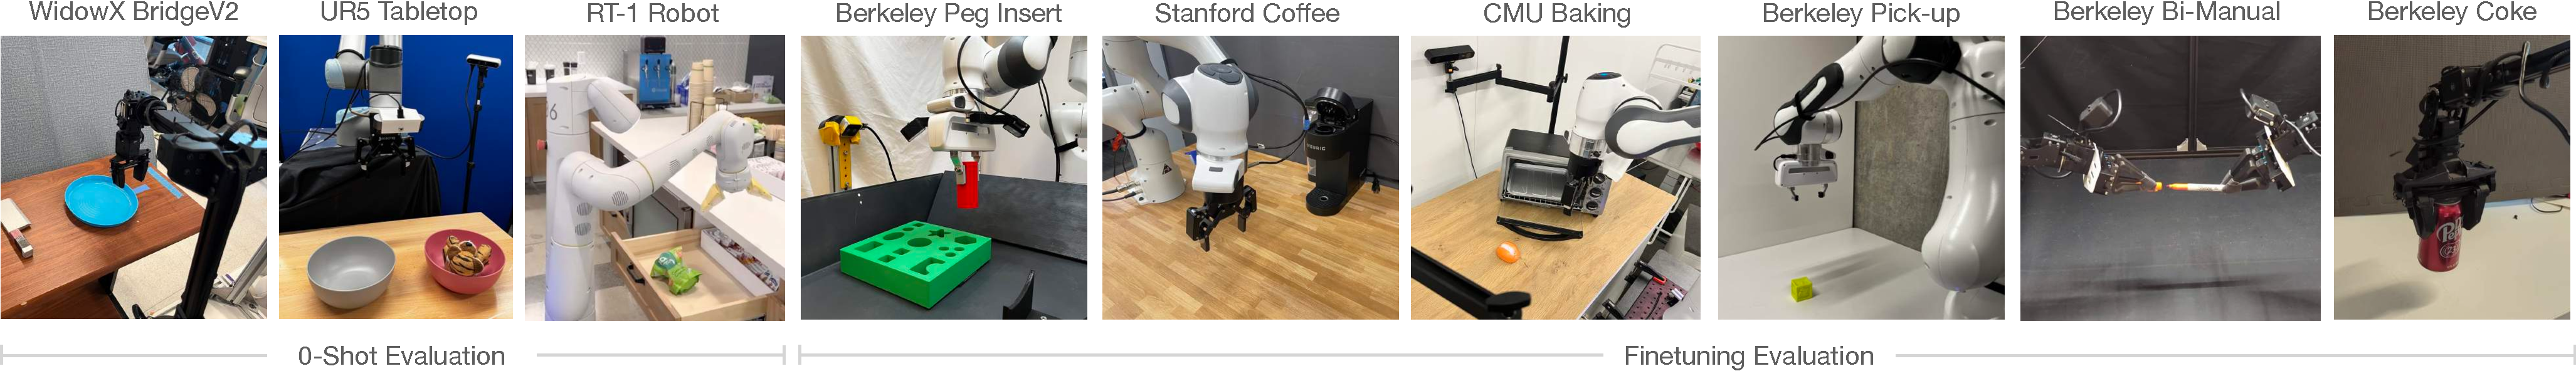
\includegraphics[width=\textwidth]{figures/orca_eval_setups_final.pdf}
    \caption{\textbf{Evaluation Tasks.} Replicated from the main text for convenience. We evaluate \method{} on \nsetups{}~real robot setups across \ninstitutions{}~institutions in zero-shot and finetuning scenarios.}
    \label{fig:eval_setups_2}
\end{figure*}

\subsection{Zero-Shot Evaluations}

\paragraph{WidowX BridgeV2} Uses the setup of \citet{walke2023bridgedata}, in which a Trossen WidowX 250 6-DOF robot performs diverse manipulation tasks. The observation consists of a single third person camera stream and the action space is end-effector position deltas. We evaluated two language-conditioned tasks in which a the robot needs to ``place the carrot on plate'', and ``put the eggplant in the pot.'' While these tasks are in-distribution, the policy must still generalize to novel object positions. We performed 10 trials per task and varied objects positions between trials.  

\paragraph{UR5} Uses the setup of \citet{BerkeleyUR5Website}, in which a UR5 robot arm performs multiple table top manipulation tasks. The observation consists of a single third person camera stream and the action space is end-effector position deltas. We evaluated twp language-conditioned tasks: picking a toy tiger from a bowl and placing it into a different bowl as well as wiping a table with a cloth. While these tasks are in-distribution, the policy must still generalize to novel object positions, distractor objects, and lighting. Since the training data was collected months ago and the robot setup was taken down and re-assembled, the policy must also generalize to other miscellaneous changes in the environment like a slightly different camera view and background. We performed 10 trials per task and varied objects positions between trials.

\paragraph{RT-1 Robot} Uses the setup of \citet{brohan2022rt}, in which a proprietary robot performs multiple table top and furniture manipulation tasks. The observation consists of a single third person camera stream and the action space is end-effector position deltas. We evaluated on the task of picking up a 7up can, apple, blue chip bag, or brown chip bag, as well as the task of opening or closing drawers on a cabinet. While these tasks are in-distribution, the policy must still generalize to novel object positions. Additionally, since the robot setup was moved between buildings, the policy must also generalize to miscellaneous changes in the environment like a slightly different camera view and background. We performed 10 trials per task and varied objects positions between trials.

\subsection{Model Ablations}
All of our model ablations were evaluated on the WidowX setup. We present a more detailed breakdown of the success rates per task in Table \ref{tab:ablations-breakdown}. We evaluated on two language-conditioned tasks (put carrot on plate and put eggplant in pot) and two goal-conditioned tasks (put bread on plate and put spoon on glove). The goal-conditioned tasks contain objects not seen in the Bridge dataset. Additionally, we analyze the generalization capabilities of Octo across several different axes, such as novel objects, novel environments and novel skills in Table \ref{tab:gen-type}.

\begin{table*}
\centering
\resizebox{\textwidth}{!}{\begin{tabular}{ccccccc}
\toprule
&& \multicolumn{2}{c}{Language-conditioned} & \multicolumn{2}{c}{Goal-conditioned} & \\
\cmidrule(lr){3-4}
\cmidrule(lr){5-6}
&& Put carrot on plate & Put eggplant in pot & Put bread on plate & Put spoon on glove & Average \\
\midrule

&\method{}-small (Ours) & 80\% & 90\% & 70\% & 90\% & \textbf{83\%} \\
\midrule

\parbox[t]{2mm}{\multirow{1}{*}{\rotatebox[origin=c]{90}{\textsc{data}}}} & RT-X dataset mix \citep{open_x_embodiment_rt_x_2023} & 80\% & 80\% & 40\% & 40\% & 60\% \\
& Single robot dataset (Bridge Data) & 20\% & 70\% & 60\% & 20\% & 43\% \\
\midrule

\parbox[t]{2mm}{\multirow{1}{*}{\rotatebox[origin=c]{90}{\textsc{policy}}}}& Discretized Action Prediction \vspace{0.13cm} \citep{open_x_embodiment_rt_x_2023} & 0\% & 20\% & 10\% & 40\% & 18\% \\
& Continuous Action Prediction (MSE) \vspace{0.13cm} & 70\% & 30\% & 0\% & 40\% & 35\% \\
\midrule

\parbox[t]{2mm}{\multirow{1}{*}{\rotatebox[origin=c]{90}{\textsc{arch}}}}& \vspace{0.4cm} Resnet-50 + Transformer \citep{open_x_embodiment_rt_x_2023} & 80\% & 60\% & 100\% & 40\% & 70\% \\
\bottomrule
\end{tabular}}

\caption{\textbf{Model Ablations.} We achieve best performance when using the ViT architecture, diffusion action head, and wide training data mixture. All evaluations are performed on the WidowX setup. Success rates are averaged over 40 trials across two language-conditioned tasks and two goal-conditioned tasks.}
\label{tab:ablations-breakdown}
\end{table*}


\begin{table*}
\centering
{
\begin{tabular}{cccc}
\toprule

Generalization Type & Task & Success Rate & Average  \\
\midrule

\multirow{2}{*}{In-distribution} & Put carrot on plate & 80\% & \multirow{2}{*}{85\%}\\
& Put eggplant in pot & 90\% \\
\midrule

\multirow{2}{*}{Novel objects} & Put bread on plate & 70\% & \multirow{2}{*}{80\%} \\
& Put spoon on glove & 90\% \\
\midrule

\multirow{2}{*}{Novel environment} & Put mushroom in pot & 20\% & \multirow{2}{*}{40\%} \\
& Put spoon on cloth & 60\% \\
\midrule

\multirow{2}{*}{Novel skill} & Flip cup on its side & 10\% & \multirow{2}{*}{5\%} \\
& Put block in slot & 0\%\\
\bottomrule

\end{tabular}}

\caption{\textbf{Zero-shot Generalization Analysis.} Using the WidowX setup, we analyze the generalization capabilities of \method-small along several different axes. \method{} performs the best on in-distribution tasks and generalizes well to novel objects and environments. However, \method{} struggles to generalize to skills not seen in the WidowX embodiment. Success rates are averaged over 20 trials across two tasks.}
\label{tab:gen-type}
\end{table*}

\subsection{Finetuning Evaluations}
\paragraph{CMU Baking} The robot must pick up the toy bread object, place it in the toaster, and shut the toaster. This task requires generalization across initial positions (of both the toaster and object) and the shape of the target toy bread object. We use an end-effector delta action space (Cartesian position + rotation delta). Observations come from the 3rd-person front-facing Zed camera. Actions are predicted at 15 Hz, and executed on the robot using the \href{https://github.com/AlexanderKhazatsky/R2D2}{R2D2 Franka controller}. The finetuning dataset consists of 120 demos collected via expert VR tele-operation, and every policy was evaluated using 20 trials (4 novel test objects with 5 positions each). 

\paragraph{Stanford Coffee} The robot is tasked with picking up one of four different Keurig Coffee Pods and placing it inside of a Keurig machine. This task requires both generalization across initial positions and colors of the coffee pod, as well as precise placement in the Keurig machine. We use an end effector delta action space with an open source controller running at 10 Hz based on Polymetis~\citep{Polymetis2021} (found \href{https://github.com/jhejna/robot-lightning}{here}). We use only a single 3rd-person wrist observation. Our training dataset contained 118 expert demonstrations from varied coffee pods and positions collected via VR tele-operation. We evaluated policies for 20 episodes, five episodes for each of four different color coffee pods.

\paragraph{Berkeley Peg Insertion} The task is to insert a pre-grasped 3D-printed peg into a matching slot on a 3D-printed board inside the bin. The matching tolerance between the peg and the hole is 1.5mm; which makes it a contact-rich precise part-mating task. 
The robot must learn an appropriate policy to ``search" for the matching opening through contact, which necessitates the use of force/torque measurements. The observation space of the policy consists of a single side-view camera image, the end-effector twist, and the end-effector force/torque reading. The policy sends action commands as the robot's end-effector twists at 5 HZ, tracked at 1000 HZ by a low-level impedance controller. Our finetuning dataset is composed of 100 human demonstrations from the FMB dataset~\citep{luo2023fmb}. We evaluated trained policies for 20 trials with randomized board positions.

\paragraph{Berkeley Pick Up} We use the setup of \citet{radosavovic2023robot}. The robot needs to pick up a block from a table top surface after being trained on a dataset of 100 pickups of various objects. The robot uses joint position control with an underlying Polymetis control stack~\citep{Polymetis2021} (\href{https://github.com/jhejna/robot-lightning}{here}). It is conditioned on a wrist camera input image, as well as the proprioceptive readings of the robot. We evaluted on the task of picking up the yellow cube and used 20 trials.

\paragraph{Berkeley Coke} A Trossen Robotics ViperX robot is tasked with picking up a coke can from a table. The ViperX is completely unseen in the training mixture, thus this task tests the model's capabilities to generalize to a new robot embodiment. The task also requires generalization across different positions of the coke can with the ViperX robot using end-effector delta control at 5Hz.
The policy uses image observations from a third person and a wrist camera. Our training dataset contained 115 expert demonstrations collected via VR tele-operation from varied positions.

\paragraph{Berkeley Bimanual} The task requires an ALOHA bimanual robot~\cite{zhao2023learning}, consisting of two ViperX robot arms, to pick up a sharpie marker with the right hand from the workbench and remove its cap with the left hand. Since \method{} was only pre-trained with single-arm robot data, we re-initialize a new action head that maps to the 14-dimensional action space of ALOHA (2x 6 joint positions + 2x gripper position). A successful policy needs to use image observations from the left and right wrist cameras to predict precise manipulation behaviors. Best performance for both our methods and baselines was achieved by predicting an action chunk of 64 during training, and then during test-time executing 12 actions with receding horizon control before re-planning. We evaluated the uncapping task using 10 trials, where the pen was placed in a different location for each trial.




\end{appendices}
